\chapter{研究方法}

\section{目標}
\begin{itemize}
	\item 該電子設備能夠測出多種腐敗產生的氣體,並且測出濃度。
	\item 該電子設備之靈敏度能高於人體嗅覺可察覺的程度,在人類鼻子無法感測到的濃度之下,
		即可發現該氣體並顯示濃度。
	\item 透過前述腐敗產生氣體的濃度,訓練出一個判斷肉品腐敗的模型,並透過模型判斷狀態,且準確率能高過 8 成。 
	\item 訓練出的判斷模型能夠與設計的硬體裝備整合,變成最終的測量裝置。
\end{itemize}

\section{方法及步驟}
\begin{enumerate}
	\item 先選定幾個腐敗時會產生的氣體,硫化氫($H_2S$)、氨氣($NH_3$)、二氧化碳($CO_2$),用不同濃度測試,確認感測器能否在鼻子還無法辨別
		的濃度下,先測出化學物質的濃度。
	\item 並透過數據推論出即將要開始壞掉的食物的數據,並以分別定義:\begin{itemize}
	 	\item 放置 0 $\sim$ 2 小時:狀態良好
		\item 放置 3 $\sim$ 6 小時:狀態尚可
		\item 放置 $>$ 7 小時:狀態不良
		\end{itemize}
	\item 累積數據,並且以數據分析,接著透過機器學習的方式訓練出一個判斷其狀態的模型。
	\item 作出一個容器用於保存肉品同時收納相關感測器設備並做出區隔,且能夠測量後顯示綠燈(食物完全沒有測出腐敗的跡象)、黃燈(食物可能有很低程度損壞)、
		紅燈(極建議丟棄)三種標示。 
\end{enumerate}

\section{實驗設備與作業環境}
	\subsection{感測器}
	\begin{itemize}
		\item MQ-136 \begin{itemize}
			\item 對硫化氫、液化氣、天然氣、城市煤氣、煙霧有較好的靈敏度
			\item 在本實驗中主要用於硫化氫感測
			\begin{figure}[H]
				\centering
				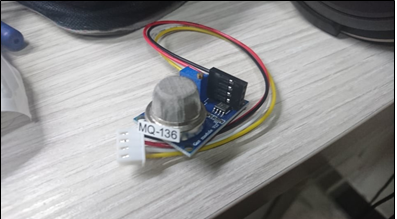
\includegraphics[width=0.5\textwidth]{../../pic/mq-136.png}
			\end{figure}
		\end{itemize}
		\item MQ-137 \begin{itemize}
			\item 對氨氣、三甲胺、乙醇胺氣體具有很高的靈敏度
			\item 在本實驗中用於測量氨氣濃度
			\begin{figure}[H]
				\centering
				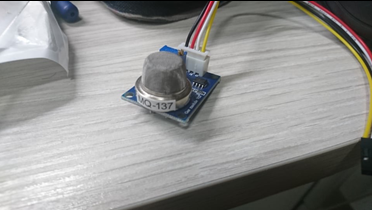
\includegraphics[width=0.5\textwidth]{../../pic/mq-137.png}
			\end{figure}
		\end{itemize}
		\item MH-Z19B \begin{itemize}
			\item 主要應用於暖通製冷與室內空氣品質監控
			\item 在本實驗用於測量二氧化碳濃度
			\begin{figure}[H]
				\centering
				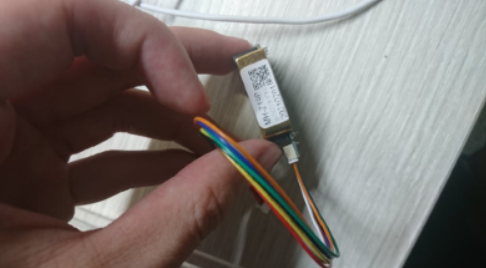
\includegraphics[width=0.5\textwidth]{../../pic/mh-z19B.png}
			\end{figure}
		\end{itemize}
	\end{itemize}
	\subsection{控制板}
	\begin{itemize}
		\item Arduino UNO R3:用於連接感測器,並執行感測器的相關讀取程式來取得需要的氣體濃度數據
		\begin{figure}[H]
			\centering
			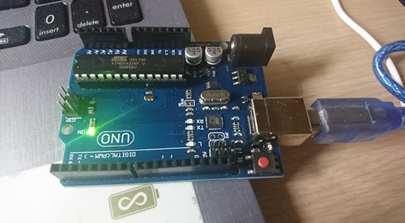
\includegraphics[width=0.5\textwidth]{../../pic/Uno.png}
		\end{figure}
	\end{itemize}
	\subsection{ML模型}
	\begin{itemize}
		\item 決策樹\\
			決策樹(英語:Decision tree)演算法採用一樹狀結構,透過一層一層的判斷來實現我們需要的分類。
			樹中每個節點表示某個特徵,而每個分叉路徑則代表某個特徵可能出現的屬性值,
			而每個葉節點則對應從根節點到該葉節點中間所經歷的路徑所表示的對象的值。
		\item SVM\\
			支援向量機(英語:support vector machine,簡稱 SVM)演算法中,若以二分類問題為例,
			我們將特徵數為 n 的資料繪製在 n 維空間中,而其不同座標的值則是對應的特徵的值,接著嘗試在這多維空間中,
			找到一個決策邊界讓兩類之間的邊界最大化,使其可以完美區隔開來,即為其分類的超平面。
			至於多分類的問題,常見的解法有一對多法和一對一法。對於有 m 個分類的資料集,一對多法是把其中的一類作為正集,
			其它的 m-1 類作為負集,這樣就把資料集分了正負兩類,以此類推會產生 m 個分類器。
			一對一法則是對於有 m 個分類的資料集,任選其中的兩類,訓練出一個分類器,以此類推總共會產生 C(m, 2) 個。
		\item 單純貝氏\\
			單純貝氏(英語:Naive Bayes)演算法是以貝氏定理為基礎,透過機率的計算,用以判斷未知類別的資料應該屬於那一個類別。
			概念是藉由分析資料中不同特徵與標籤之間發生的機率,並以此作為分類的依據。
		\item AdaBoost\\
			自適應增強(英語:Adaptive Boosting,簡稱 AdaBoost)是一種迭代算法,在每一輪中加入一個新的弱分類器並更改資料的權重,
			直到達到某個預定的足夠小的錯誤率或迭代次數。每一個訓練樣本一開始都被賦予一個相同的權重,
			之後經過弱分類器分類後,已經被準確地分類的樣本權重會降低,反之錯誤的權重會增加,
			權重改變後資料集會被用於訓練下一個弱分類器,如此迭代地進行下去。
			最後將所有弱分類器組合成強分類器。各個弱分類器的訓練過程結束後,增加誤差率小的弱分類器的權重,
			反之降低誤差率大的弱分類器的權重,使其在最終的分類函數中起著較大的決定作用。
	\end{itemize}